\documentclass[12pt, twocolumn, a4paper]{article}
\usepackage[top=2cm, bottom=2cm, outer=2cm, inner=2cm]{geometry}
%\usepackage[pages=all]{background}
\usepackage{comment}
\usepackage{textcomp}
\usepackage{fontspec}
\usepackage{setspace}
\usepackage{lastpage}
\usepackage{fancyhdr}
\pagestyle{fancy}
\usepackage{graphicx}
\graphicspath{ {./images/} }

%\backgroundsetup{
 %   scale=1,
 %   color=black,
 %   opacity=1.0,
 %  angle=0,
 %   contents={%
 %     
\includegraphics[width=\paperwidth,height=\paperheight]{lol.jpg}
 %     }%
%}
\singlespacing
\title{\textbf{%NANYANG RESEARCH PROGRAMME \\
Low-cost alternatives to Proton Exchange Membranes in Microbial Fuel Cells for use in education}}
%
%\author{
    %\begin{tabular}[t]{c@{\extracolsep{7em}}c} 
    %Akshay Parthasarathy,  & Dr. Timothy TM Tan, \\
    %Kuan Zhi Xun, &  National Institute of Education\\ 
    %Temasek Junior College & \\
    %\end{tabular}
%}
\author{Akshay Parthasarathy, \\ Kuan Zhi Xun \\ EY018
%\\  Temasek Junior College
}
\date{}

\begin{document}
\maketitle
\begin{abstract}
    The use of microbial fuel cells (MFCs) in integrated science, technology, engineering, and mathematics (STEM) education has become increasingly popular in education circles. The MFC uses interdisciplinary scientific concepts to harness electricity from respirating microbes. However, to enable widespread educational use of MFCs, using Nafion\texttrademark{} membranes is impractical. In this study, our objective was to investigate the feasibility of using cheaper materials as the membrane in an MFC as a cost-effective alternative to the expensive standard membrane, using a modified version of the conventional Bennetto MFC; Parchment Paper, Cellophane, Dialysis Tubing; as well as aluminum, plastic, and filter paper as negative controls. We also tested rudimentary treatment with PVA glue to decrease chemical and physical permeability to electrons and substances other than protons, as well as to increase the productivity of MFC by increasing the effectiveness of charge balancing between chambers. The result we got shows that the best candidate is double-layered parchment paper, having shown a comparable peak in average open circuit voltage (OCV) and only a 49. 1\% reduction in the average lifespan duration from those when Nafion\texttrademark{} is used, compared to the 72.7\% decrease for the other membrane candidates, in addition to outperforming Nafion\texttrademark{} for more than 3 hours on average. Thus, we have achieved our goal of finding a low-cost alternative to expensive Nafion\texttrademark{} membranes. Further studies are required on the inexplicable and inconsistent performance of aluminum foil as a membrane in MFCs.
\end{abstract}
\section{Introduction}
\paragraph{}The use of microbial fuel cells (MFCs) in integrated science, technology, engineering and mathematics (STEM) education has seen an increasing popularity in education circles. The MFC applies interdisciplinary scientific concepts to harness electricity from respirating microbes. Taking advantage of the blend of intertwining scientific workings and design variability of the MFC, schools can organize programs to enrich students' learning. One such MFC design-based inquiry program was outlined by Tan and Lee, 2022. \cite{educsci12060417} However, a significant obstacle in the adoption of MFC technology as a teaching tool lies in its cost. The standard for proton exchange membranes (PEMs) in MFCs is the Nafion\texttrademark{} membrane, which costs between US\$1500 to US\$3100 per square meter, possibly the most cost-effective component. \cite{costnafion} This makes adopting MFCs unsustainable for lab use in most schools as they are restricted by budget constraints. The problem is further exacerbated due to the tendency of students to make mistakes or the necessity to repeat the prototyping process during experiments. \cite{experimentationandeducation} 

\paragraph{}Membranes in MFCs act as separators between the cathode and anode chambers. In industrial and research applications, PEMs are utilised with the membrane allowing, theoretically, only $H^{+}$ cations (protons) across to the cathode chamber. \cite{Kusoglu2017} By nature, these proton exchange membranes consist of membrane backbones treated chemically to contain negatively charged groups. \cite{cole1972membranes} This serves the dual purpose of allowing the passage of positively charged protons, but also preventing the flow of anions and electrons across the chambers. \cite{Hickner2004} The effectiveness of this technology was underscored when DuPont invented "Nafion" membranes, which increased the efficiency of fuel cells by a magnitude of 4. However, to enable widespread educational use of the MFCs, using Nafion membranes is impractical. 

\section{Aims and Objectives}
\paragraph{}Through this study, we aim to investigate the feasibility of using cheaper materials as the membrane of the MFC. In order to increase the suitability of adopting MFCs as a teaching tool, we aim to develop a simple, inexpensive method for the production of the membrane, such that it is reproducible within the confines of school laboratories. This considerably lowers the barrier for implementation of effective MFC-based learning programs in schools. Thus, we will be studying the effectiveness of different common partially permeable membranes in replacing the PEM in a modified version of the conventional Bennetto MFC as a cost-effective alternative to the expensive standard Nafion\texttrademark{} membrane.
\section{Hypothesis}
\paragraph{}We have identified the following membrane materials for investigation. 
        \begin{center}
        \begin{table}[h]
        \begin{tabular}[H]{ |c|c| } 
         \hline
         {\small\textbf{Name}} & {\small\textbf{Cost}} {\footnotesize(US\$ per $m^2$)}\\
             \hline
             {\small Nafion} & {\small 1500 - 3100}\\
             {\small Cellophane} & $\approx$ {\small 2.00}\\
             {\small Baking Paper} & {\small 2.50}\\
             {\small Dialysis Tubing} & {\small$\approx$ 1600}\\
         \hline
         
        \end{tabular}
        \caption{Cost comparison of different Membrane Candidates}
        \end{table}
        \end{center}
    \paragraph{}Cellophane is a promising material for our purposes. It is readily available, partially permeable at 0.11 $kg\cdot m^{-2} \cdot h\cdot bar$ to 0.23 $kg\cdot m^{-2} \cdot h\cdot bar$ \cite{Makarov2022}. Additionally, Azizul et al. have found that cellophane works well as a membrane in a no-moisture MFC design. \cite{MOQSUD20132465} The paper found that cellophane was "not reusable due to it deteriorating quickly", which may be an area of concern for us. However, given that cellophane is extremely cheap, using cellophane as a disposable membrane has significantly greater suitability than Nafion\texttrademark{} PEMs in the context of schools, due to the cost factor and the fact that only a small 6 $cm$ by 6 $cm$ membrane is needed per MFC.
    
    \paragraph{}As dialysis tubing is double layered cellophane, it will be interesting to note whether the precisely controlled pore size has any effect on the membrane. Although, dialysis tubing usually come with a relatively narrow breadth of about 4.5 $cm$, it is still sufficient to prevent leakage of reagents across the chambers of an MFC; we will still cut the dialysis tubing membrane sample that are 6 $cm$ in length.

   \paragraph{}Fraiwan and Choi \cite{C4CP04804K} have found parchment paper (better known as baking paper) to be suitable for use as a paper-based PEM, producing a "maximum power of 10 $\mu A cm^{-2}$ at a current density of 50 $\mu A cm^{-2}$ as compared to when Nafion is used.  This was attributed to parchment paper's ability to block most anolytes and catholytes from permeation through the parchment paper membrane. Despite the fact that Fraiwan and Choi were researching an air cell MFC, this is relevant to our project since the air cell MFC operated in the same principles as a liquid reagent-based Bennetto MFC cell. This finding is supported by Choi et al.'s \cite{C5AN00492F} research into a '48-well on printed circuit board' MFC design, which used the same operational principles of a liquid reagent-based MFC. The open circuit voltage (OCV) values obtained, which "ranged from 570 to 618 $mV$", were substantial, relative to the size of the wells as chambers for the reagents. Lee et al. \cite{Lee2016-xq} were able to produce substantial OCV results of 302 $mV$ with their "micro-fabricated solvent-free air cathode all-paper MFC". They credited the parchment paper PEM to be able to "pass only H+ from the anode to the cathode", which meant that parchment paper is a suitable material to conduct only protons through itself \cite{doi:10.1021/acs.chemrev.6b00159}, rendering the material a theoretic good fit for our project's aim. We have opted to use Baking Paper available off the shelf in supermarkets.
\section{Methodology}
\paragraph{}For the negative controls, we chose to do a 3-hour run as a proof of concept. We used Aluminium Foil (Diamond Heavy Duty Aluminium Foil, Embossed Foil, 7.6 $m$ x 45.7 $cm$), Plastic from a new Ziploc bag (Ziploc® Brand Freezer Bags Quart, 7 $in$ x 8 $in$), and filter paper (Whatman® Grade 3 Qualitative Filter Paper, Standard, 125 $mm$ Circle, 100 Pack). Our expectation was for 0 $V$ to be recorded for both Aluminium Foil and Plastic, and for filter paper to peak at a lower OCV and for a shorter period of time than the other membrane materials tested due to its relatively high permeability.

\paragraph{}We then tested the suitability of the different membrane materials as the PEM in an MFC through a series of experiments: 
    \begin{enumerate}
        \item Using a single layer to mimic the standard MFC set up with the Nafion\texttrademark{} membrane
        \item Using a double layer to decrease physical permeability to substances other than protons to increase the productivity of the MFC, by increasing the effectiveness of charge balancing between chambers, as well as to increase the longevity of the MFC OCV level by strengthening the structural integrity of the PEM unit
        \item Using a single layer soaked in glue (PVA) solutions to decrease chemical and physical permeability to electrons and substances other than protons, to increase the productivity of the MFC by increasing the effectiveness of charge balancing between chambers
    \end{enumerate}
    \subsection{Procedures}
        \paragraph{}MFC kits originally desgined by Bennetto \cite{bennetto1990electricity} were used with modifications and alternative reagents \cite{educsci12060417} better suited to a school environment. In particular, each cell will consist of cathode and anode chambers separated by a membrane, and these chambers are fitted with a carbon fibre electrode each. In the anode chamber, 3.0 $mL$ of 1.0 $M$ Glucose, 3.0 $mL$ of 0.01M Methylene Blue in 0.1 $M$ Phosphate buffer, 3 $mL$ of yeast slurry. Yeast slurry is prepared by placing 1.5 $g$ dried instant Baker's Yeast in a clean, dry centrifuge tube, and adding 10 $mL$ of 0.1 $M$ Phosphate Buffer and gently stirring it till the yeast is rehydrated. The cathode chamber will have 9 $mL$ of 0.02 $M$ Potassium Permanganate solution instead of Potassium ferricyanide as described in Bennetto's paper on MFCs. All reagents used are prepared in 0.1M Phosphate buffer ($pH$ 7.0) to maintain a consistent neutral pH environment in the cell for the yeast to function optimally. 
        
        \paragraph{}We measured OCV values over time using voltage sensors measuring ±1.0 $V$ connected to a datalogger. We were able to collect OCV values for 3 MFC runs together with internal temperature of the cells per datalogger (4 channels). Internal temperature was recorded such that we could monitor potential temperature chnages while the MFC runs were left overnight, which may affect the OCV values read by the voltage sensor. For experimentation with different membrane material candidates, OCV values were collected "1 Data per 1 $Min$" (Very Slow Sampling) for 24 hours (overnight). Meanwhile, OCV values were collected "1 Data per 10 $Secs$" (Very Slow Sampling) for the 3-hour negative controls experiment. After each MFC run, we saved the data collected by the datalogger in Comma Separated Values ($.csv$) format in an Secure Digital (SD) card before exporting to Microsoft Excel for data analysis.
        
        Preparation of Glue Solution:
        \begin{enumerate}
                \item Add 0.5 $mL$ of PVA white glue (Clag® Kids PVA 236 $mL$) each to 2 clean, dry 15 $mL$ centrifuge tubes using a clean, dry 1 $mL$ syringe. Label the 2 centrifuge tube as “Distilled Water Diluted” and “Phosphate Buffer Diluted” respectively.
                
                \item Add enough distilled water to the “Distilled Water Diluted” centrifuge tube with 0.5 $mL$ glue to make up 10 $mL$ of 20x diluted glue solution.
                
                \item Repeat step 2 with the “Phosphate Buffer Diluted” centrifuge tube by adding 0.100 $M$ phosphate buffer ($pH$ 7.0) instead of distilled water.
                
                \item Shake and mix the contents of the 2 centrifuge tubes well to make uniformly diluted glue solutions
        \end{enumerate}
        

        Preparation of Glue-Soaked Membranes:
        
        1. Use a clean, dry glass rod to dip into the “Distilled Water Diluted” glue solution and evenly spread out on both sides of the different membrane material samples (as many as required).
        
        2. Store the glued membranes individually between sheets of cling wrap to allow the membrane to absorb the glue (where applicable) and for the glue to dry overnight
        
        3. Repeat step 1-2 for membrane samples to be soaked in the “Phosphate Buffer Diluted” glue solution

    \subsection{Data Analysis}
        \paragraph{}Data analysis will be carried out using two comparisons conducted, one on performance over time within the same type of membrane, and the other being the comparison between peaks of the plotted average OCV curves from different membrane candidates. The best membrane candidate will exhibit both a high peak comparable to Nafion\texttrademark{}, and last for a significant period of time.
    
\section{Results / Discussion}
    \begin{figure}
        \centering
        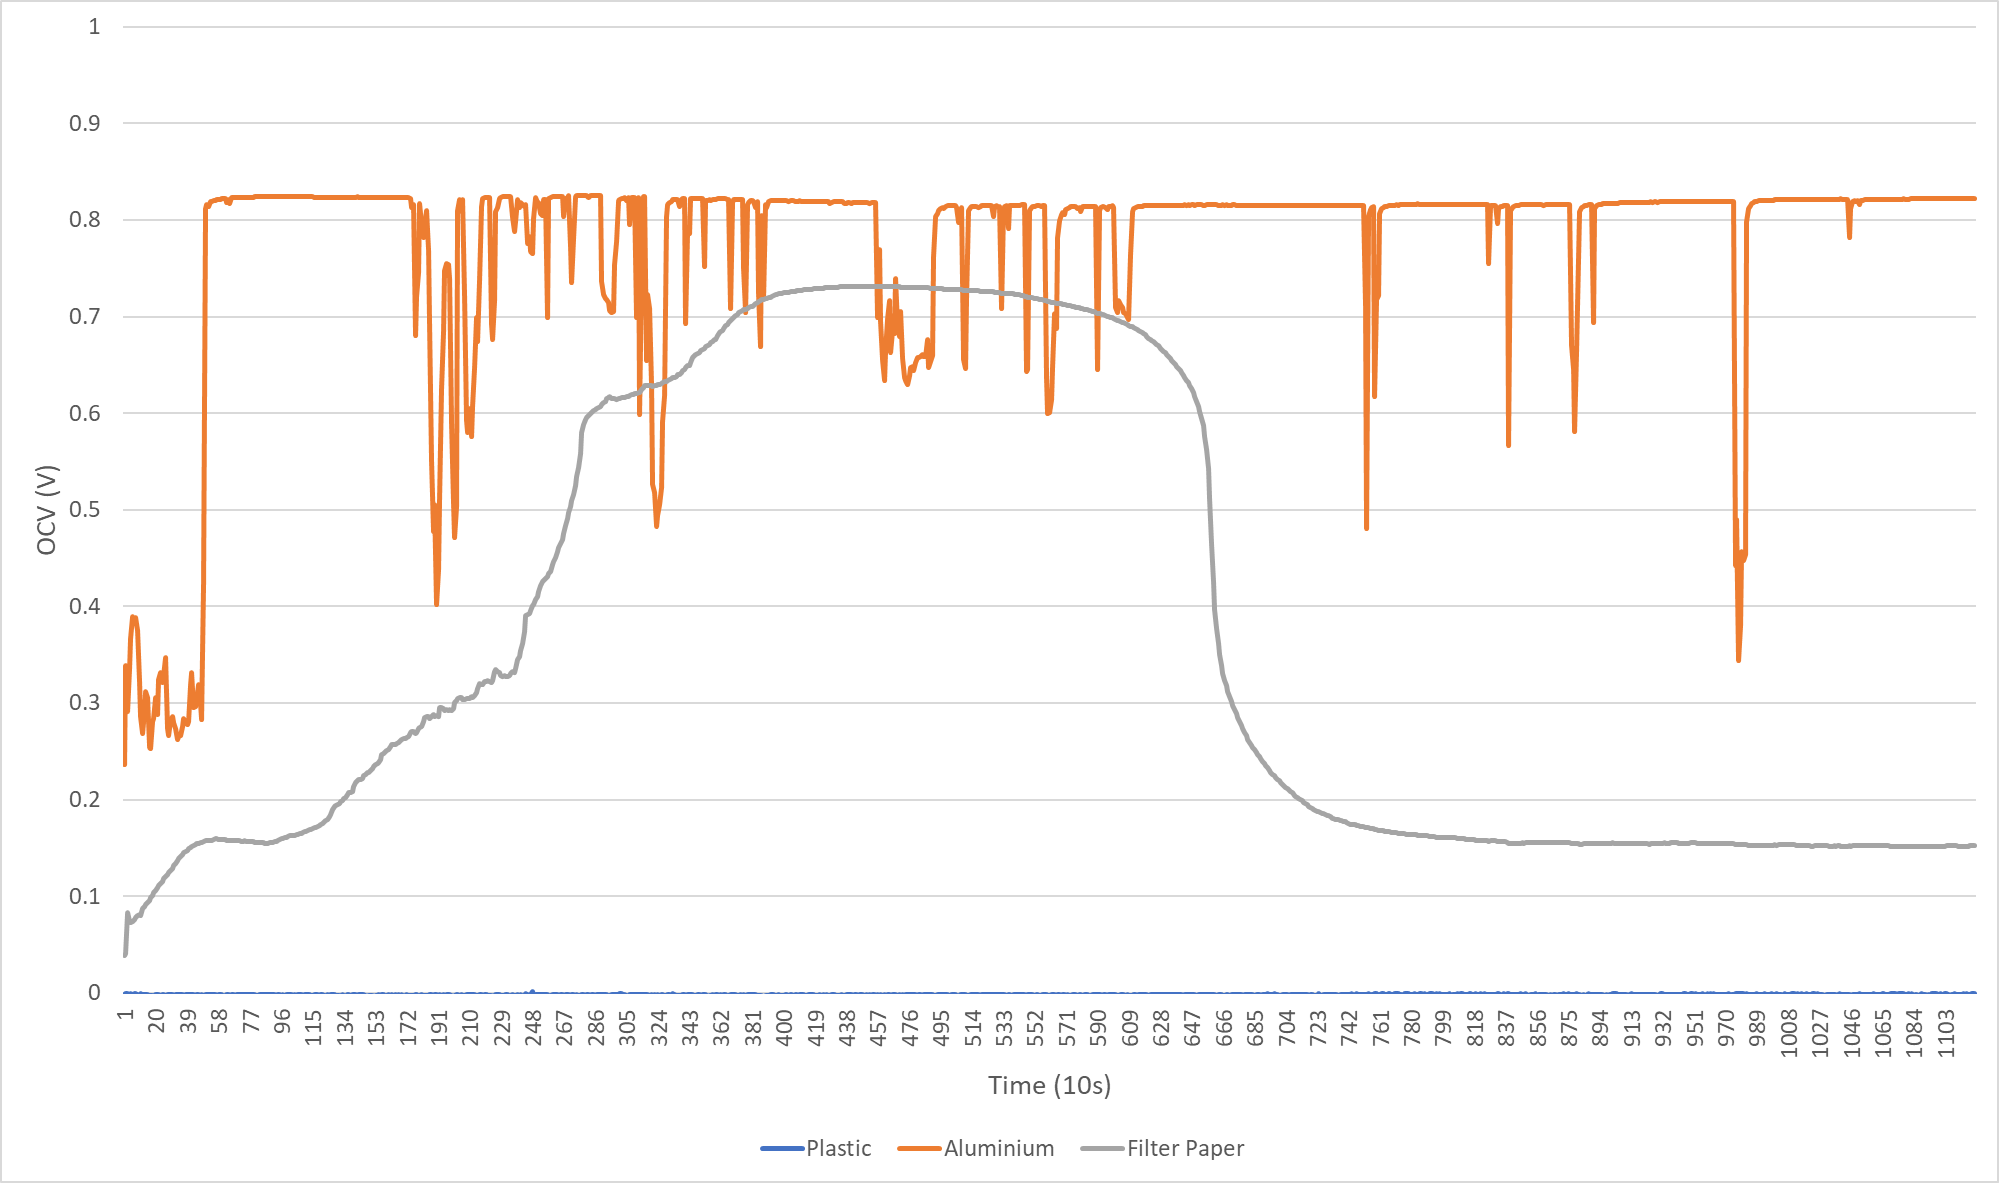
\includegraphics[scale=0.25]{negative controls.png}
        \caption{Short run experiment using negative controls detailed in section 3.}
        \label{fig:averages}
    \end{figure}
    \paragraph{}Looking at the results in Figure 1 on negative controls, for plastic and filter paper, the results obtained match our expectations. However, it is Aluminium that produces inexplicable results. Theoretically, as aluminium is not a permeable membrane, protons cannot pass from the anode chamber to the cathode chamber, and no OCV should be recorded. Further, as a conductor of electrons, what we expected to observe was a short circuit, and hence, a $0V$ reading on the Voltmeter.
    \begin{figure}
        \centering
        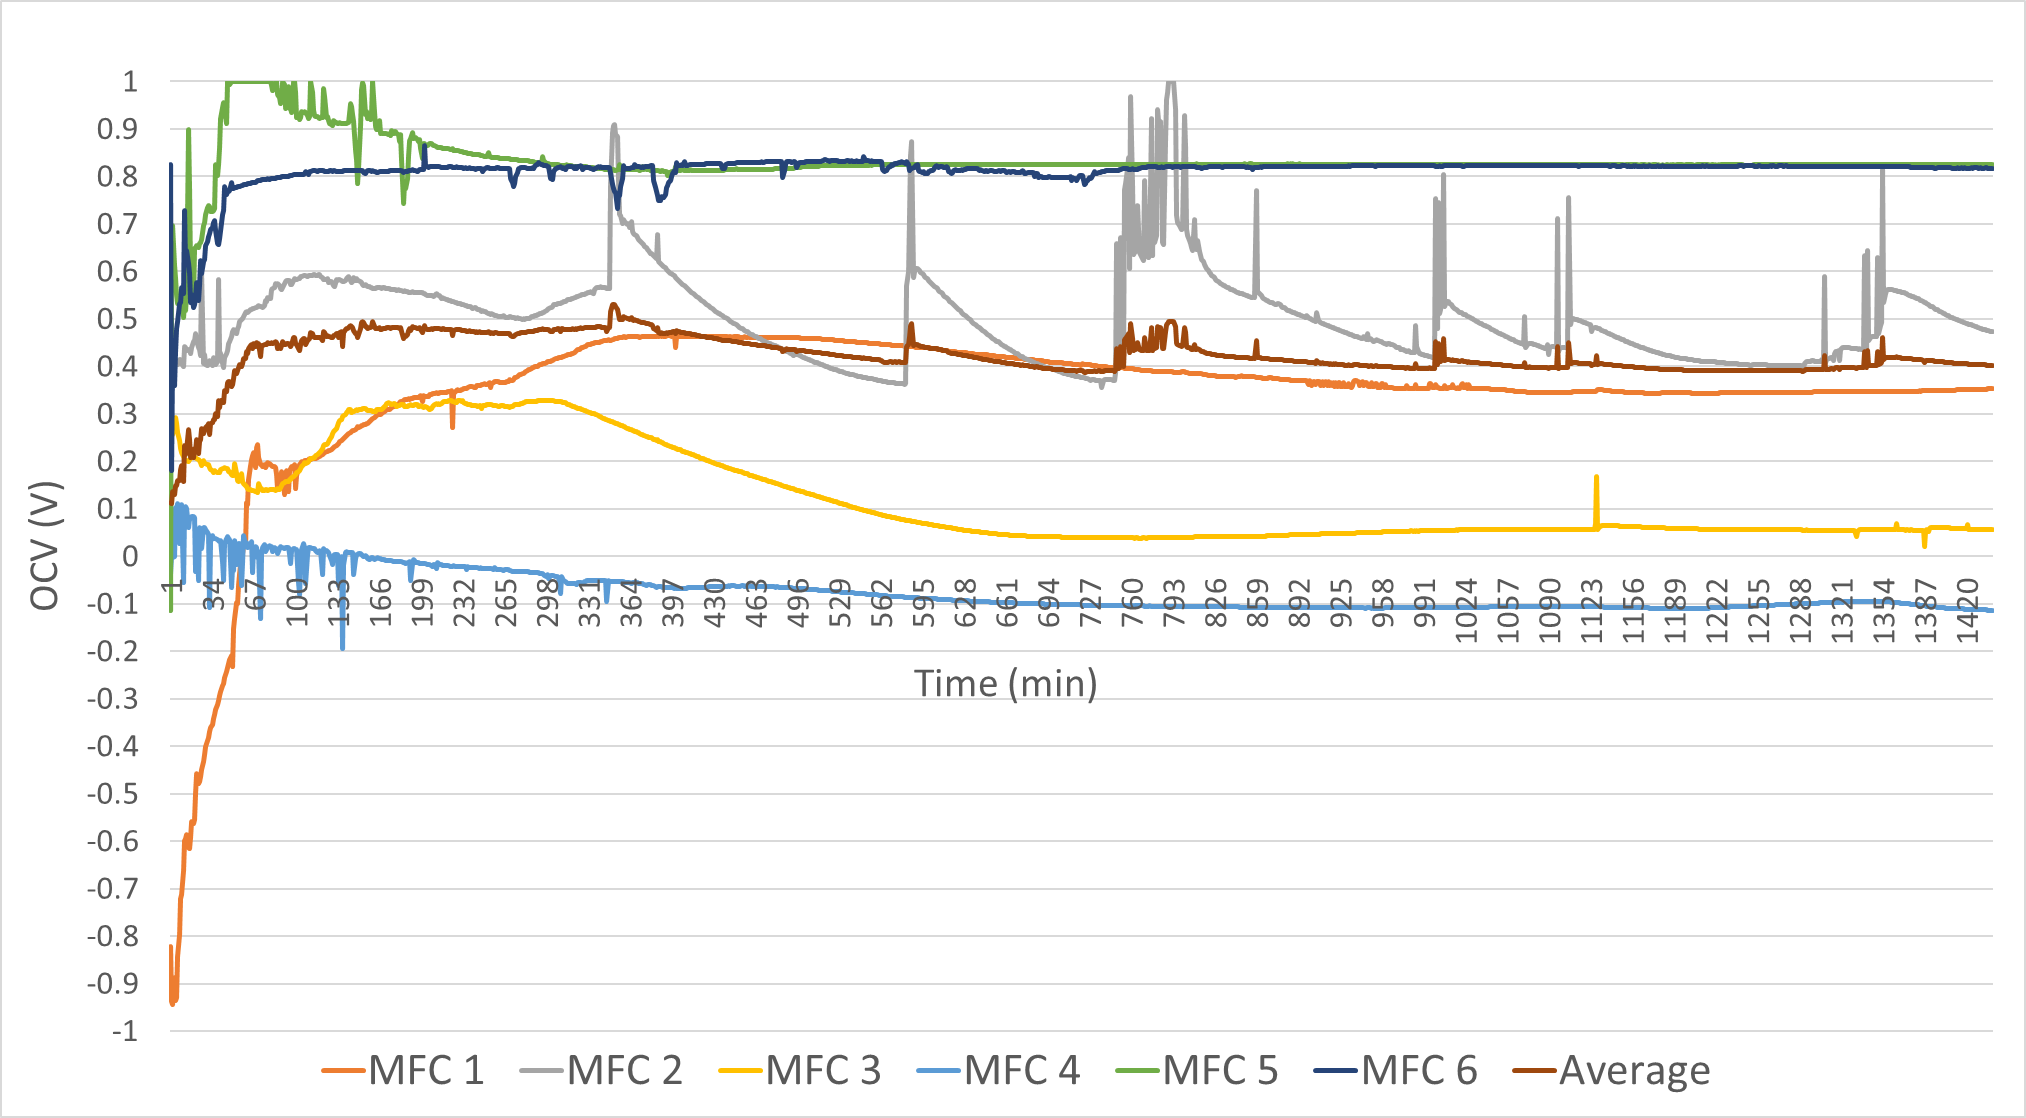
\includegraphics[scale = 0.25]{aluminium.png}
        \caption{Graph of the 6 runs with aluminium as a membrane.}
        \label{fig:my_label}
    \end{figure}
    \paragraph{}As seen in Figure 2, only MFC 3 and 4 gave predicted results of low longevity and OCV peak at about 0.328 $V$ and effectively 0 $V$ output respectively. These are expected because aluminium foil is not permeable to protons and are unable to balance the charge on both chambers in the long run. However, for the other MFC runs with conflicting results, for which there are no satisfactory explanation based on current knowledge. We have come up with a few possible hypothesis: 
    \begin{enumerate}
        \item The aluminium ($Al$) in aluminium foil membrane sample was oxidised by the potassium permanganate solution in the cathode chamber of the MFC into non-conductive Aluminium oxide solids, blocking electrons from passing from the anode chamber directly to the cathode chamber through the aluminium foil membrane sample. This would force electrons to pass through the electrodes and the voltage sensors to give positive OCV readings instead of 0 $V$ readings.
        \item The carbon fibre electrodes were touching the aluminium foil membrane sample in the MFC, which would have led to the electrons of the aluminium foil entering the circuit, giving rise to a positive OCV reading.
        \item $Al$ in aluminium foil membrane sample somehow displaced a less reactive metal to form aluminium cations ($Al^{3+}$), which can balance the charge between both chambers. 
        \item There is an issue with voltage measurement considering the low OCV in the MFC [unlikely because the OCV for plastic from a Ziploc bag was low and effectively zero as excepted]
        \item The MFC does not work like we thought it does.
    \end{enumerate}
\paragraph{}We suspect that the electrical conductivity of Aluminium probably plays a significant role in the highly unexpected and unpredictable results. We expect that using electrically conductive materials like aluminium foil as a PEM in MFCs will likely give rise to similar variable and fluctuating results. We reused the same Voltmeters as the other materials, and they produced reliable results before and after testing with Aluminium. Consequently, it is our belief that equipment failures are not to blame, and further, deeper examination is required.

    \begin{figure}
        \centering
        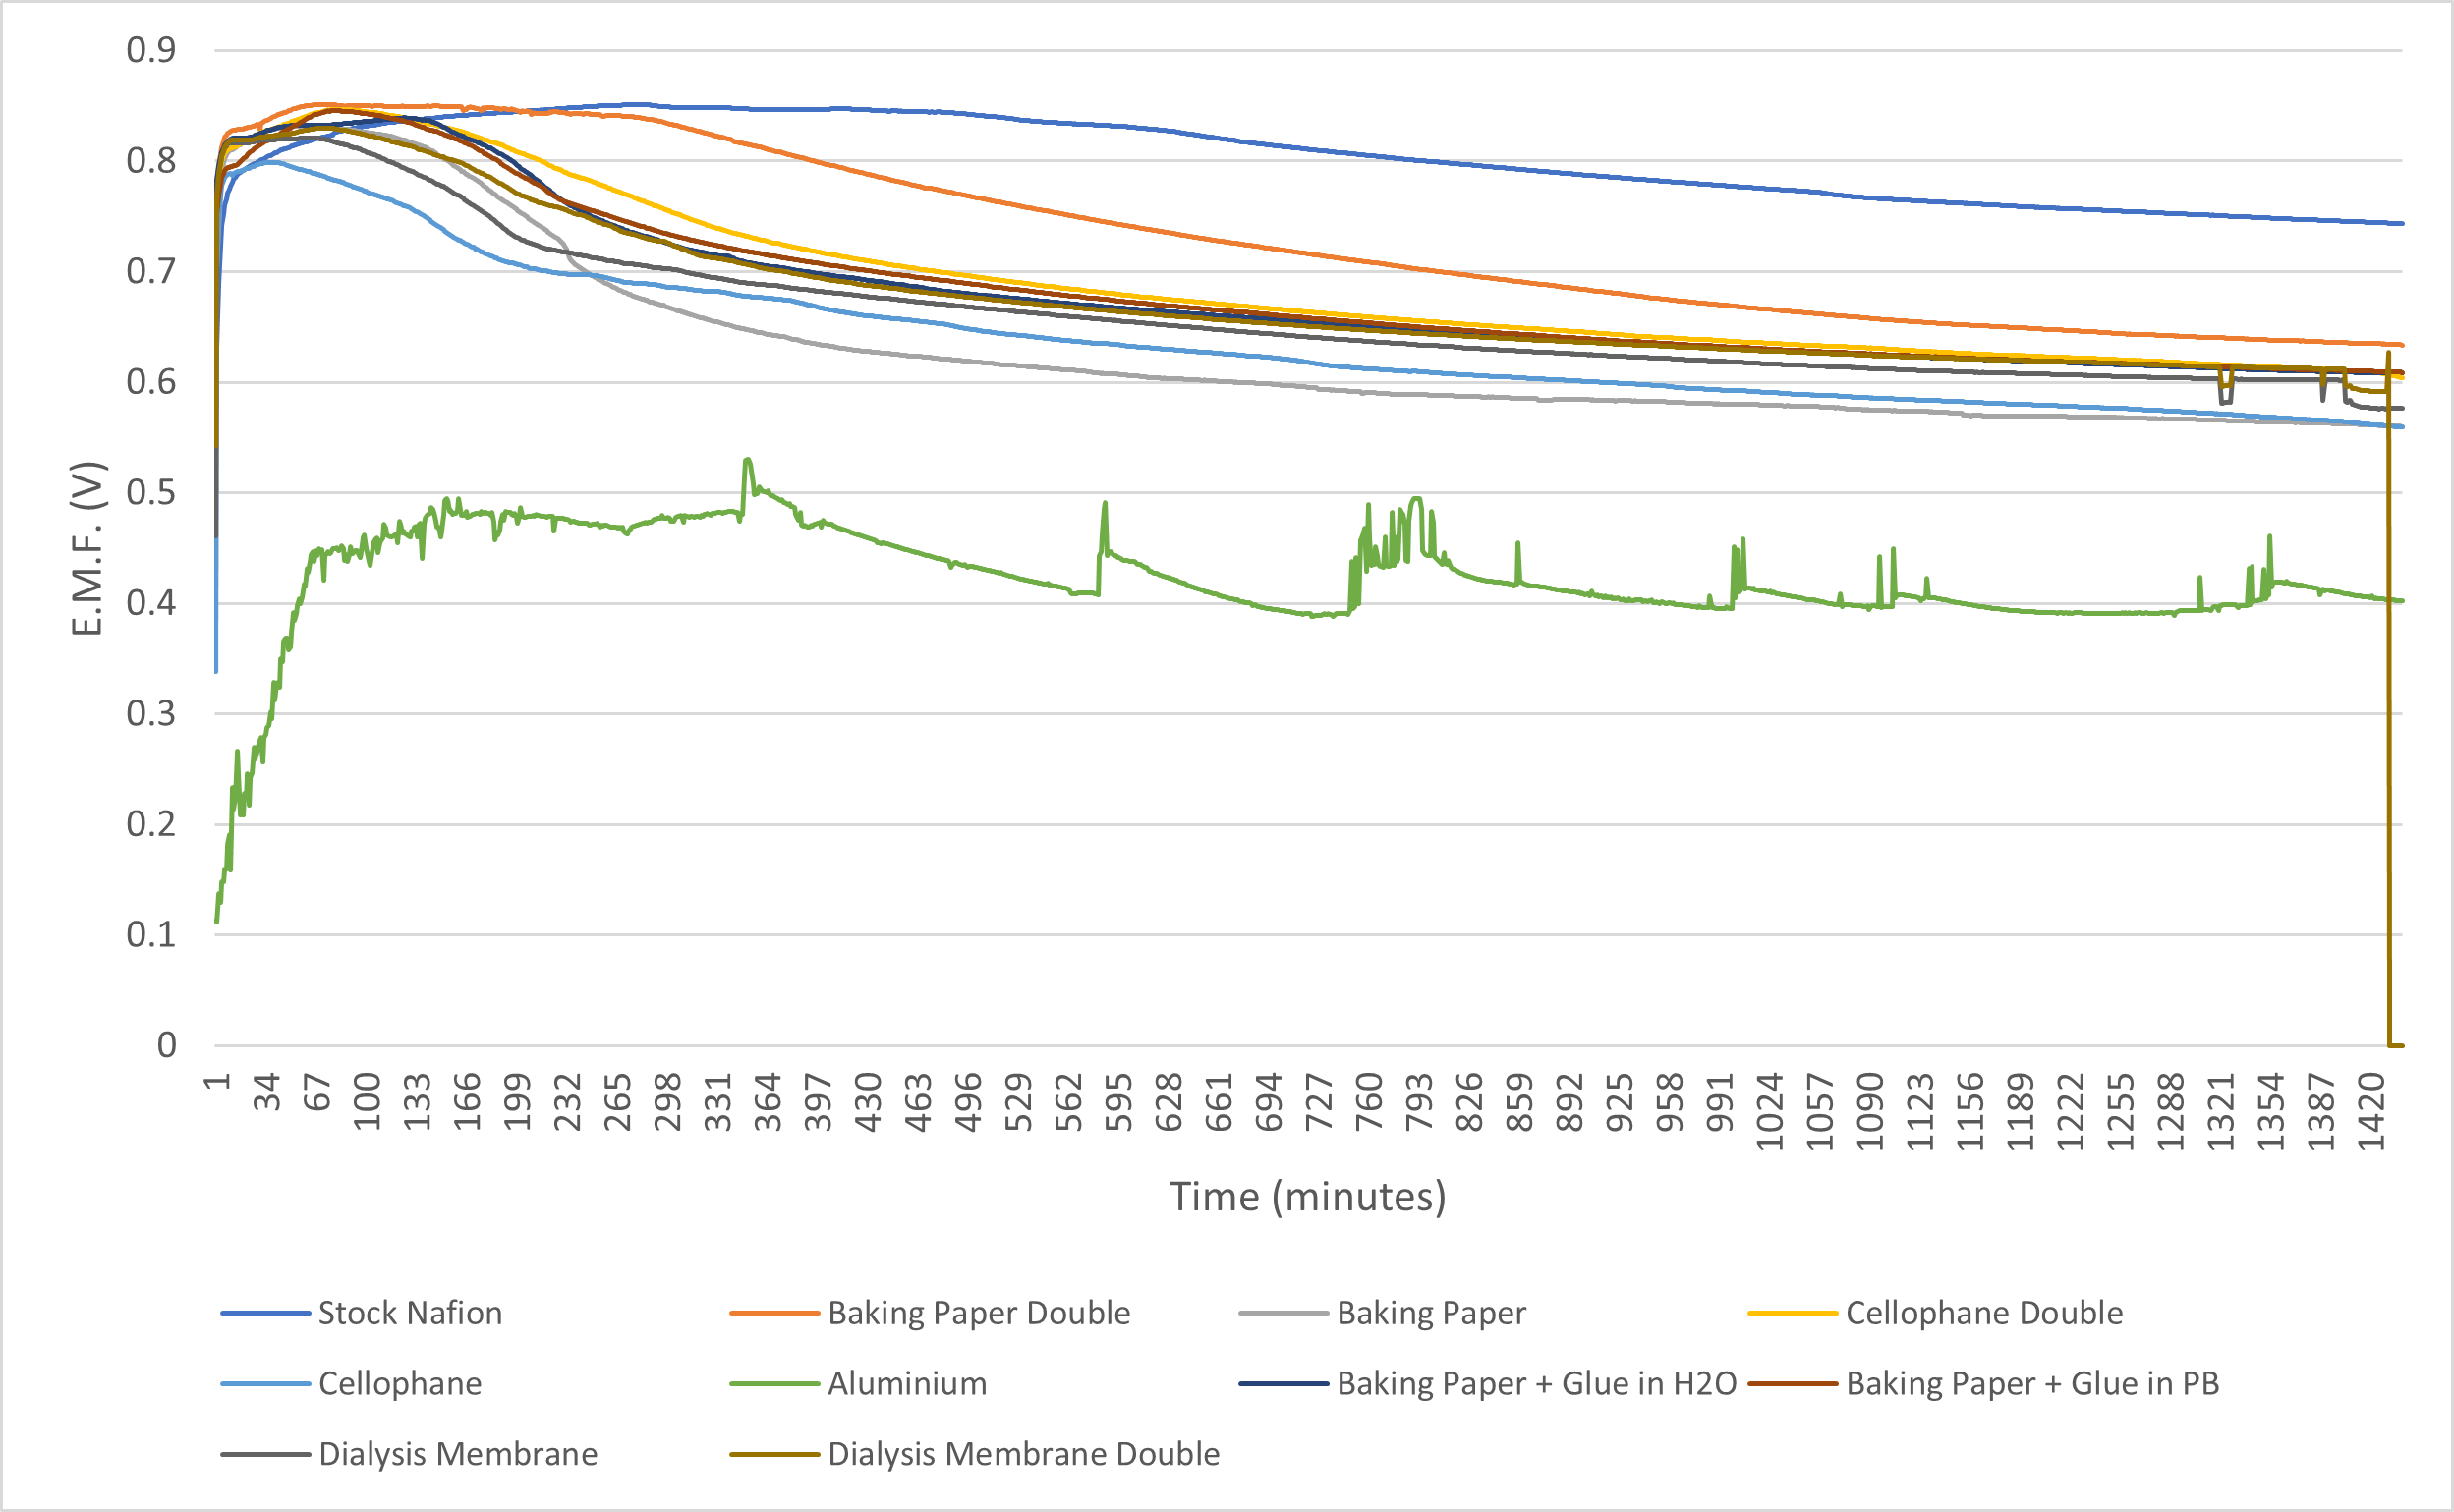
\includegraphics[scale = 0.2]{Averages.png}
        \caption{Average OCV produced from all runs of each type of membrane used}
        \label{fig:averages}
    \end{figure}
    \begin{figure}
        \centering
        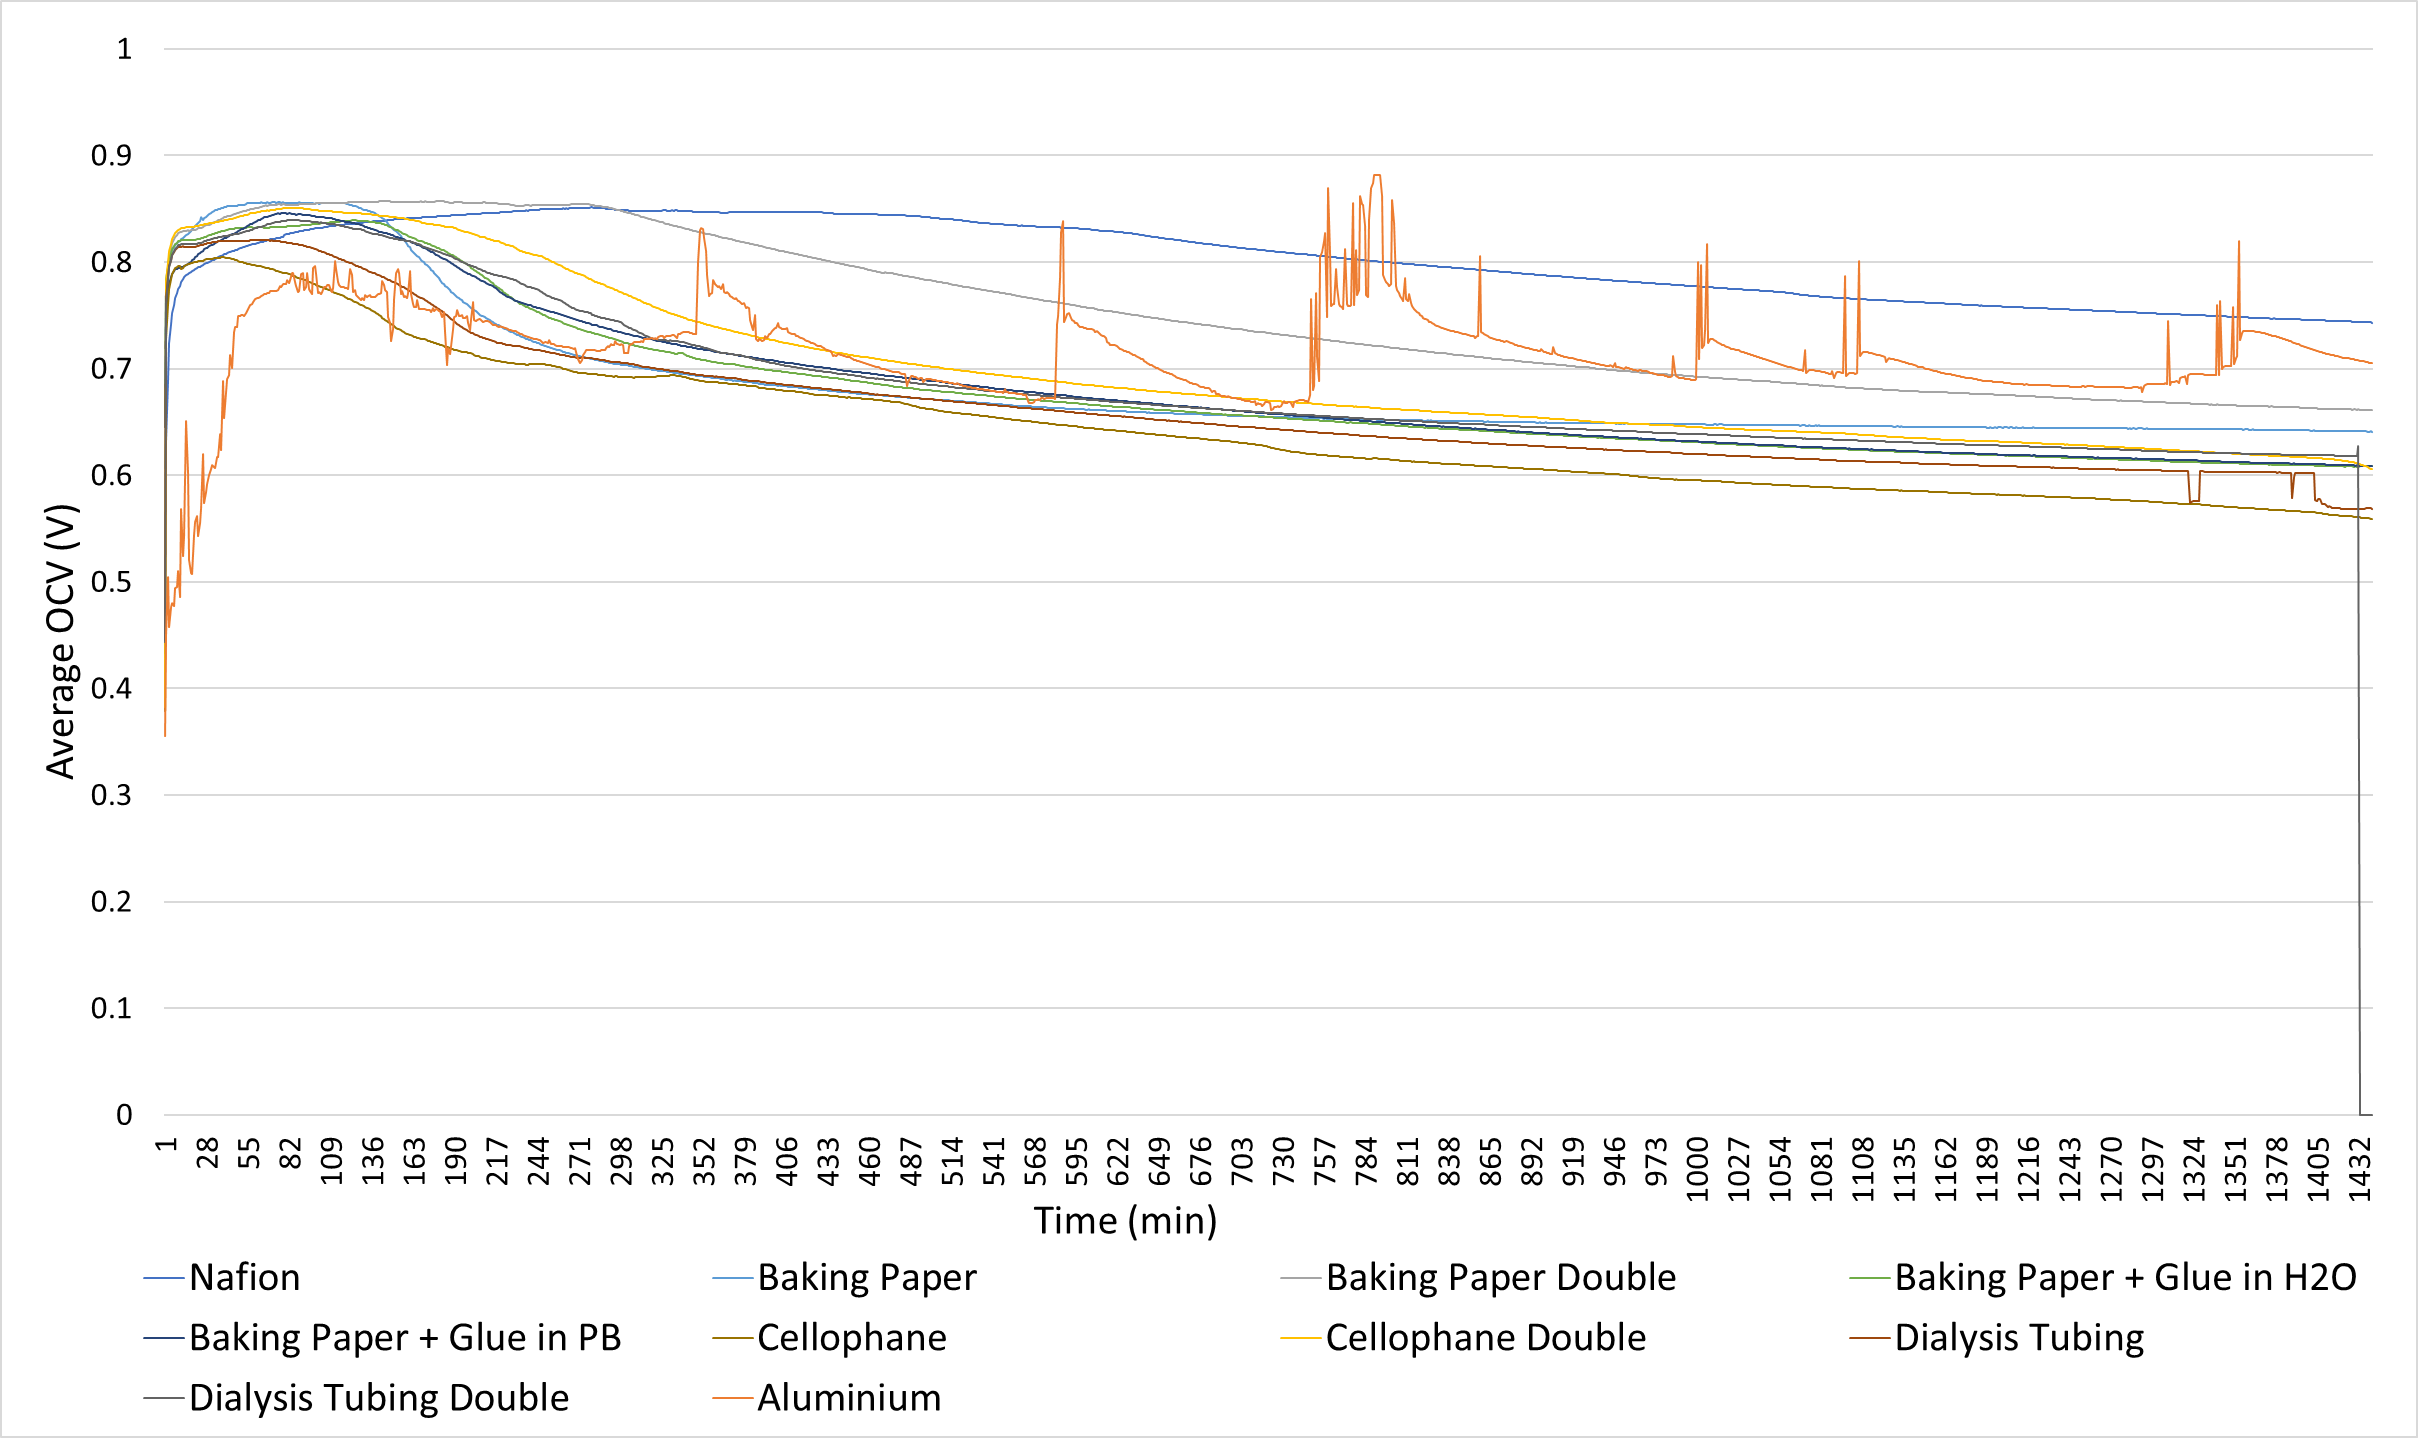
\includegraphics[scale=0.2]{best3.png}
        \caption{Average OCV produced from the best 3 runs of each type of membrane used}
        \label{fig:averages}
    \end{figure}
    
    \paragraph{}It is evident that, overall, Nafion\texttrademark{} remains as the best performing membrane material candidate; average OCV peaked at a high of about 0.851 $V$ and had an OCV ≥ 0.800 $V$ for 12.8 hours after 29 minutes. The next best candidate is double layered parchment paper which peaked at about 0.851 $V$ and had a average OCV ≥ 0.800 $V$ for 6.5 hours after 3 minutes. The most interesting result is that the double layered parchment paper outperforms Nafion\texttrademark{} up until the 3.4 hour mark before falling off. On the other hand, taking the 3 best runs for double layered Baking Paper, we found that it outperformed Nafion\texttrademark{} in terms of average OCV value for almost 5 hours before it was outperformed. 
    
    \paragraph{}For cellophane, double layering provides an $\approx5.3\%$ increase in recorded OCV values, while for baking paper, double layering improved recorded OCV values by $\approx2.3\%$. Overall, the double layering the membranes produced significantly better results while soaking in Glue solution made up with phosphate buffer resulted in an $\approx1.6\%$ improvement, greater than the $\approx0.8\%$ improvement provided by soaking in Glue solution made up with $H_{2}O$. This shows that double layering the membrane was more effective in decreasing permeability to substances and reagents not including protons than PVA treatment, as double layering a material increases the physical reinforcement by splitting the contact point of reagents to the PEM into 2 different sheets of the same membrane material. 
    \paragraph{}Within the glue-soaked parchment paper runs, we expected the glue solutions prepared in different solvent bases (phosphate buffer and distilled water) to give approximately equal increase in performance. However, this difference (p<0.05) indicates that the solvent base does make a difference in results. We propose that this difference in results was caused by the introduction of more negatively-charged phosphate ions (${PO_{4}}^{3-}$) through the glue solution diluted in phosphate buffer. Anions like ${PO_{4}}^{3-}$ can electrochemically associate with the basic R-groups of the cellulose in parchment paper via the formation of hydrogen bonds \cite{PBIthing}. This association confers the membrane material a greater overall slight-negative charge that will repel electrons, which could explain the difference in results when glue solutions prepared in different solvent base are used. 

    \paragraph{}Cellophane was the worst performing of the lot, peaking at 0.799 $V$ and not producing a average OCV ≥ 0.800 $V$. This is expected considering that cellophane does not undergo significant processing in its manufacturing like parchment paper (siliconisation of both sides of the paper) and dialysis tubing (standardisation of pore size). Dialysis tubing showed a $\approx2.0\%$ higher peak and double layering had a $\approx3.2\%$ increase on cellophane. This however is an expensive improvement on cellophane, given that the price of dialysis membranes can rival Nafion\texttrademark{}.
    
\section{Conclusion}
\paragraph{}Our results show that there are indeed suitable alternative MFC PEM materials, the best alternative of which is double layer parchment paper, having showed a comparable peak in average OCV and only a 49.1\% reduction in average longevity duration from when the Nafion\texttrademark{} is used, compared to the ≥ 72.7\% reduction in average longevity for the other membrane material candidates. The reality is that with only a 49.1\% decrease in MFC longevity, students receive a more accurate view of the lifespan of an MFC. Taking the cheapest cost per $m^2$ of Nafion\texttrademark{} as the standard cost rate of the use of Nafion\texttrademark{} in an MFC, there would be a 99.7\% decrease in cost of a PEM for every MFC that uses double layer parchment paper as a PEM. Integration of PEMs into science classes would be more accessible.

\paragraph{}Our results also confirmed that the excellent performance of parchment paper (with respect to its cost) as a PEM in alternative MFCs described in the literature \cite{C4CP04804K, C5AN00492F, Lee2016-xq}, translated into great performance in our modified-for-school-usage MFC setup. This is cause for greater confidence in general in the assumption that results of our particular MFC setups can apply and translate relatively well to other MFC setups that operate on the same principles; in our case, a 2-chambered reduction-oxidation- (redox-) powered proton exchange MFC cell.

\paragraph{}Our results on aluminium, to the best of our knowledge, have no explanation through the currently accepted principles of the functioning of an MFC. Further research is required as to whether Aluminium Foil truly works, albeit inconsistently, in place of the Proton Exchange Membrane, and provide an alternative explanation for this effect or show that the data obtained is an outlier.
%There is actually another high-cost barrier in this version of the MFC, which is the use of expensive carbon fibre tissue as electrodes in the cell. While alternatives to carbon fibre electrodes are not investigated in this project, we hope to see future publications prying into this matter. This way, as the cost of implementing this version of an MFC would decrease further, students would have a higher chance of benefiting greatly from studying the concept of an MFC.

\section*{Acknowledgements}
\paragraph{}We are extremely grateful for the opportunity to work on an interesting and engaging project through the Nanyang Research Programme. We would like to thank Dr Tan Ter Ming Timothy for providing us with the essential chemicals, space in his laboratory at the National Institute of Education, Singapore, and most importantly, his valuable time spent mentoring us in the ways of research. Lastly, we would like to extend our gratitude to Temasek Junior College for its support and our Teacher-Coordinator, Mrs Aileen Lim for her understanding and supervision, which were instrumental in our project.

\footnotesize
\bibliography{test}
\bibliographystyle{ieeetr}
\end{document}
